\chapter{Theoretical overview}
\label{chap:refs}


\section{Introduction}\label{sec:introduction}

The development of a custom Virtual File System (VFS) with versioning and encryption capabilities requires an understanding of several key concepts and technologies.
This chapter aims to provide the necessary background and context to deeper understand the VFS implementation discussed in later chapters.
Even for those already familiar with the subject, a brief refresher might be helpful.


\section{Understanding File Systems}\label{sec:file-systems}

Let's start with what a file system is and what it does, as it is important for understanding the VFS itself.

A file system is a critical component of any operating system, tasked with managing and organizing data stored on a device.
As described by Oja et al.~\cite{oja-fs}, a filesystem represents the methods and data structures used by an operating system to maintain files on a disk or partition, that is, how files are organized on the disk.
This consist of multiple operations such as creation, reading, modifying, and deleting files or directories.
This is done in order to allow users and applications to interact seamlessly with the underlying storage medium.

It is important to distinguish between a disk or partition and the file system it contains.
While some programs operate directly on raw disk sectors or partitions, which could potentially damage or corrupt existing file systems, most programs interact with a file system.

There are various types of file systems, each tailored for specific operating systems and purposes.
Notable file systems include NTFS (New Technology File System) for Windows, HFS+ for macOS, and ext4 (fourth extended filesystem) for Linux.
Cross-platform compatibility can be attained using universal file systems like FAT32 or exFAT, which are compatible with multiple operating systems.

File systems employ diverse techniques to organize data, such as partitioning, allocation units, and indexing.
Additionally, file systems manage metadata, which is crucial for organizing and accessing stored data.
Metadata encompasses information such as file names, creation and modification timestamps, file sizes, and access permissions.


\section{Virtual File Systems}\label{sec:virtual-file-systems}

A Virtual File System (VFS) is an essential abstraction layer in modern operating systems, designed to ease the interaction between various file systems and user applications.
The VFS functions as an intermediary, enabling applications to access various file systems through a unified interface, regardless of the underlying file system's specific characteristics or structure.

According to a book by David A. Rusling~\cite{rusling-linux}, the VFS manages various mounted file systems by maintaining data structures that describe the entire virtual file system and the real mounted file systems.
The VFS uses superblocks and inodes, similar to the EXT2 file system, to describe files and directories within the system.
Each file system registers with the VFS during operating system initialization.
File system modules are loaded as needed, allowing VFS to read their superblocks.
The VFS maintains a list of mounted file systems and their VFS superblocks, with each superblock containing pointers to specific file system functions.
he VFS efficiently maps information for various file systems, including EXT2.

The VFS inodes are traversed as the system's processes access directories and files.
Frequently accessed inodes are kept in the inode cache for quicker access.
Additionally, the Linux file systems use a common buffer cache, independent of the file systems, to cache data buffers from underlying devices.

The VFS plays a critical role in operating system design as it not only offers file system independence, but also provides benefits such as improved security or better performance.
In this thesis, I will also demonstrate that the extensibility of the VFS is a valuable advantage, enabling the incorporation of advanced features without requiring kernel modifications.

\subsection{VFS Operations}\label{subsec:vfs-operations}

The Virtual File System (VFS) provides a range of operations to interact with files and directories.
These operations are implemented as system calls, such as \texttt{open(2)}, \texttt{stat(2)}, \texttt{read(2)}, \texttt{write(2)}, and \texttt{chmod(2)}, which are called from a process context.
The VFS operations can be grouped into three main categories: directory entry cache (dcache), inode object, and file object operations~\cite{vfs}.

\textbf{Directory Entry Cache (dcache)} operations deal with the translation of pathnames (filenames) into specific dentries.
The VFS uses the dcache to implement system calls like \texttt{open(2)}, \texttt{stat(2)}, and \texttt{chmod(2)}.
Dentries exist only in RAM for performance reasons and are not saved to disk.

\textbf{Inode Object} operations involve filesystem objects such as regular files, directories, and other entities.
Inodes can reside on disk (for block device filesystems) or in memory (for pseudo filesystems).
When required, inodes on disk are copied into memory, and changes are written back to disk.
Inodes can be referenced by multiple dentries, for example, through hard links.

\textbf{File Object} operations pertain to files opened by a process, also known as ``open file descriptions'' in POSIX terminology.
File objects are represented by the \texttt{struct file\_operations} structure, which contains a variety of member functions that define how the VFS can manipulate an open file, such as reading, writing, and closing files.

To perform a specific operation on a file, the VFS first translates the user-space file descriptor into the appropriate file structure and then calls the required file structure method.
As long as the file is open, the corresponding dentry and VFS inode remain in use~\cite{vfs}.


\section{FUSE}\label{sec:fuse}

FUSE (named after Filesystem in Userspace) is an open-source software interface that allows developers to create custom file systems in user space without the need for kernel modifications.
It operates by providing a bridge between the kernel's VFS layer and user-space file system implementations.
The kernel communicates with the user-space file system using a well-defined API, allowing developers to create file systems without the need for kernel-level programming.
This abstraction greatly simplifies the development process and reduces the risks associated with kernel modifications.

To develop a new file system using FUSE, a handler program connected to the provided libfuse library must be created.
The primary objective of this handler program is to define the file system's behavior in response to read, write, and stat requests.
Additionally, the handler program is responsible for mounting the new file system.
Upon mounting, the handler is registered with the kernel.
When a user initiates read, write, or stat requests for the newly mounted file system, the kernel forwards these I/O requests to the handler, which processes them accordingly.
The handler's response is then relayed back to the user by the kernel, ensuring a seamless interaction between the custom file system and the operating system.

The FUSE flow-chart diagram created by Wikipedia user named Sven~\cite{fuse-diagram} depicted in Figure~\ref{fig:fuse-diagram} effectively illustrates the process involved in handling a command like `ls', from its initial submission to the Virtual File System (VFS) layer, through the FUSE kernel module, to a handler program in user space and back.

\begin{figure}[ht]
    \centering
    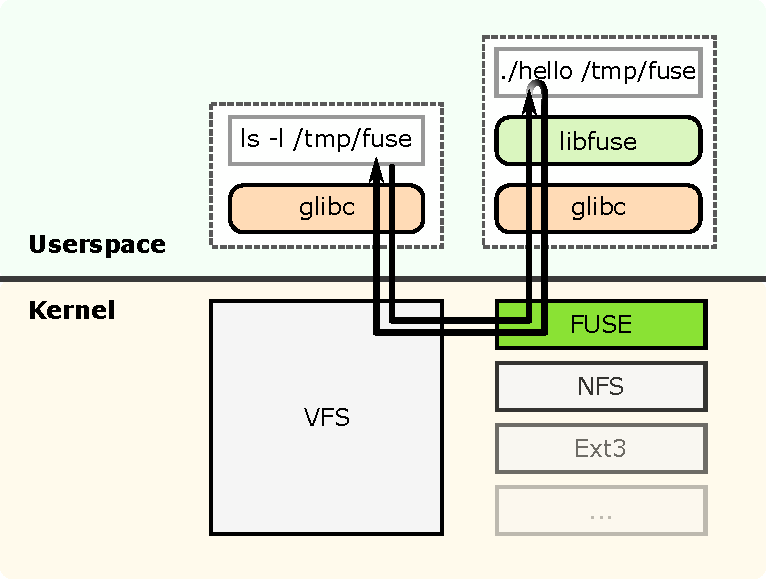
\includegraphics[width=\linewidth]{img/fuse_diagram}
    \caption{FUSE flow-chart diagram}\label{fig:fuse-diagram}
\end{figure}

FUSE has gained widespread adoption due to its ease of use and modularity.
Many popular file systems have been implemented using FUSE, such as SSHFS, GlusterFS, S3FS and NTFS-3G, among others.
These implementations demonstrate the versatility and robustness of the FUSE framework in handling a wide range of file system requirements.


\section{Encryption}\label{sec:encryption-approaches}

In this thesis, I will mainly use encryption as a process of applying cryptographic algorithms to transform the contents of files and directories into an unreadable format, which can only be deciphered with the appropriate decryption key.
Utilizing encryption enables users to effectively safeguard their data against unauthorized access, data breaches, and other malicious activities.

Within the scope of file and directory encryption, symmetric key algorithms, such as the Advanced Encryption Standard (AES), might be employed due to their computational efficiency and robust security properties.
To generate the encryption key from a user-provided password, password-based key derivation functions (PBKDFs), including bcrypt, scrypt, or Argon2, could be leveraged.


\section{Versioning}\label{sec:versioning}

Versioning is a technique used to maintain multiple copies or states of a file or directory, allowing users to access and restore previous versions as needed.
It enables tracking of changes made to files over time, facilitating collaboration and recovery from accidental data loss or corruption.

Usually, versioning is implemented by storing multiple copies of a file or directory, each representing a different version.
This approach is straightforward and easy to implement, but it can be inefficient in terms of storage space and performance.
To address these issues, versioning can be implemented using a snapshot-based approach, which stores only the differences between versions, rather than storing multiple copies of the same file.